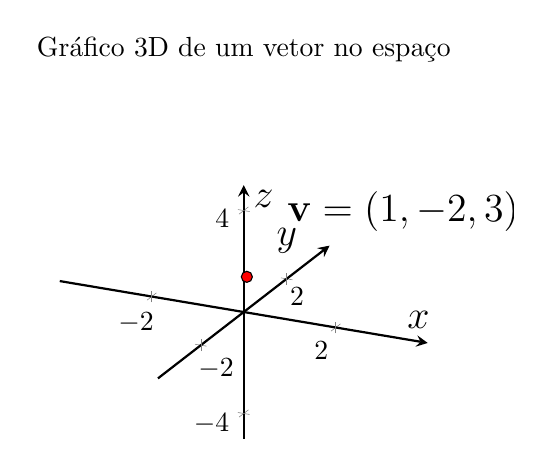
\begin{tikzpicture}
    \begin{axis}[
        axis lines = center,
        axis line style={thick},
        xlabel = {\Large $x$},
        ylabel = {\Large $y$},
        zlabel = {\Large $z$},
        xtick={-2,0,2},
        ytick={-2,0,2},
        ztick={-4,0,4},
        xmax = 4, xmin = -4,
        ymax = 4, ymin = -4,
        zmax = 5, zmin = -5,
        title={\normalsize Gráfico 3D de um vetor no espaço},
        grid=none
    ]
        % Desenhar ponto (1, -2, 3)
        \addplot3[
            only marks,
            mark=*,
            mark options={scale=1, fill=red},
        ] coordinates {(1, -2, 3)};
        % Mover o valor do rótulo para frente
        \node at (axis cs:1.9, -2.5, 5) [anchor=south west] {\Large $\mathbf{v} = (1, -2, 3)$};

        % Desenhar linhas tracejadas até os eixos
      %  \addplot3[dashed, thick] coordinates {(0, -2, 3) (1, -2, 3)};
      %  \addplot3[dashed, thick] coordinates {(1, 0, 3) (1, -2, 3)};
      %  \addplot3[dashed, thick] coordinates {(1, -2, 0) (1, -2, 3)};
    \end{axis}
\end{tikzpicture}
